Unless otherwise noted, point estimates include percentile bootstrap 95\% CIs ($B=1000$, seed~42) from the frozen prediction package.
The \textbf{primary} cross-generator metric is \textbf{UFD Macro AUC}; \textbf{OOD Pooled AUC} is supplementary only.

\subsection{Overall In-Distribution and Out-of-Distribution Performance}
\label{sec:overall}

Table~\ref{tab:overall} summarizes ID AUC, UFD Macro AUC, worst-generator AUC, and efficiency descriptors for \textbf{Panel~A} (training-matched compact models).
Table~\ref{tab:external} reports \textbf{Panel~B} external pretrained references on the same frozen manifests.

On the ID test set ($n=400$), LiteSSM-A and LiteSSM-B achieved AUCs of \textbf{0.946} $[0.926,\ 0.964]$ and \textbf{0.945} $[0.924,\ 0.964]$.
EfficientNet-B0 followed at \textbf{0.929} $[0.905,\ 0.951]$.
LiteFreqNet~v2, MobileNetV3-Small, and ShuffleNetV2-x0.5 obtained \textbf{0.906}, \textbf{0.890}, and \textbf{0.880}.
Paired bootstrap differences indicated that LiteSSM-A exceeded EfficientNet-B0 and LiteFreqNet~v2 on ID AUC ($\Delta$AUC $+0.018$ and $+0.040$; CIs excluding zero), whereas the LiteSSM-A--LiteSSM-B ID gap was negligible ($\Delta$AUC $+0.001$, CI including zero).

Under \textbf{UFD Macro AUC}, LiteSSM-A ranked first in Panel~A at \textbf{0.718} $[0.707,\ 0.730]$, followed by LiteSSM-B (\textbf{0.700} $[0.688,\ 0.711]$).
Among CNN baselines, ShuffleNetV2-x0.5 reached \textbf{0.674}, EfficientNet-B0 \textbf{0.667}, LiteFreqNet~v2 \textbf{0.645}, and MobileNetV3-Small \textbf{0.636}.
Worst-generator AUC remained near chance for every Panel~A model (\textbf{0.451--0.519}), always corresponding to DALL·E (Section~\ref{sec:ufd}).

Panel~B references attain substantially higher UFD Macro (UnivFD \textbf{0.948}; NPR \textbf{0.976}) using large-scale CLIP pretraining or official artifact-training releases; these numbers contextualize absolute room for improvement and are \emph{not} ranked against Panel~A under a shared training protocol.

\begin{table}[H]
\caption{Panel~A: controlled compact models trained under our frozen from-scratch protocol.
Efficiency numbers are from one locked RTX~4090D session (PyTorch~2.3, CUDA~12.1, FP32): batch-1 latency with $\ge$50 warmup / 500 timed iterations and CUDA synchronize (model-only; p50 shown); Thr@32 is images/s at batch size~32 in the same session.
CI intervals are 95\% bootstrap intervals for ID and UFD Macro.\label{tab:overall}}
\scriptsize
\setlength{\tabcolsep}{3.2pt}
\begin{tabularx}{\textwidth}{@{}P{2.15cm}c*{7}{R}@{}}
\toprule
\textbf{Model} & \textbf{Arch} & \textbf{Params} & \textbf{FLOPs} & \textbf{B1 p50} & \textbf{Thr@32} & \textbf{ID} & \textbf{UFD} & \textbf{Worst} \\
 &  & (M) & (G) & (ms) &  & AUC & Macro & AUC \\
\midrule
LiteSSM-A & SSM & 1.74 & 0.705 & 144.4 & 226 & 0.946 & 0.718 & 0.504 \\
LiteSSM-B & SSM & 2.48 & 0.853 & 237.6 & 120 & 0.945 & 0.700 & 0.483 \\
EfficientNet-B0 & CNN & 4.01 & 0.414 & 6.64 & 4338 & 0.929 & 0.667 & 0.519 \\
LiteFreqNet~v2 & CNN+FFT & 1.13 & 0.180 & 6.15 & 4747 & 0.906 & 0.645 & 0.451 \\
MobileNetV3-S & CNN & 1.52 & 0.061 & 4.30 & 7231 & 0.890 & 0.636 & 0.455 \\
ShuffleNet-x0.5 & CNN & 0.344 & 0.044 & 6.21 & 4817 & 0.880 & 0.674 & 0.467 \\
\bottomrule
\end{tabularx}
\end{table}

\begin{table}[H]
\caption{Panel~B: external pretrained reference detectors (inference-only).
Public weights and native preprocessing; not training-matched competitors.\label{tab:external}}
\scriptsize
\setlength{\tabcolsep}{4pt}
\begin{tabularx}{\textwidth}{@{}P{1.7cm}L*{4}{R}@{}}
\toprule
\textbf{Detector} & \textbf{Pretrained} & \textbf{Params} & \textbf{B1 p50} & \textbf{ID} & \textbf{UFD Macro} \\
 &  & (M) & (ms) & AUC & AUC \\
\midrule
UnivFD~\cite{ojha2023ufd} & CLIP ViT-L/14 & 427.6 & 11.86 & 0.608 & 0.948 \\
NPR~\cite{tan2024npr} & Official release & 1.44 & 2.89 & 0.947 & 0.976 \\
\bottomrule
\end{tabularx}
\end{table}

\subsection{Accuracy--Efficiency Trade-Off}

Figure~\ref{fig:pareto} plots UFD Macro AUC against \textbf{batch-1 latency} (ms/image; model-only, FP32, GPU synchronized; log $x$-axis); marker size encodes parameter count.
Batch-32 throughput remains reported in Table~\ref{tab:overall} for server batching and is not used as a single-image latency proxy.
MobileNet/ShuffleNet and LiteFreqNet occupy the low-latency region (about 4--7\,ms) with lower or mid-range UFD Macro.
EfficientNet-B0 is similarly fast at batch~1 ($\approx$6.6\,ms) but heavier (4.01\,M) with lower UFD Macro than either SSM.
LiteSSM-A achieved the highest UFD Macro AUC among the controlled compact models while retaining a batch-32 throughput of \textbf{226} images/s (batch-1 p50 \textbf{144.4}\,ms).
LiteSSM-B is slower (p50 \textbf{237.6}\,ms; throughput \textbf{120} images/s) with a slightly lower Macro.
LiteSSM-A is therefore selected as the preferred generalization--efficiency operating point among protocol-matched models, rather than as a real-time or lowest-latency detector.

\begin{figure}[H]
\centering
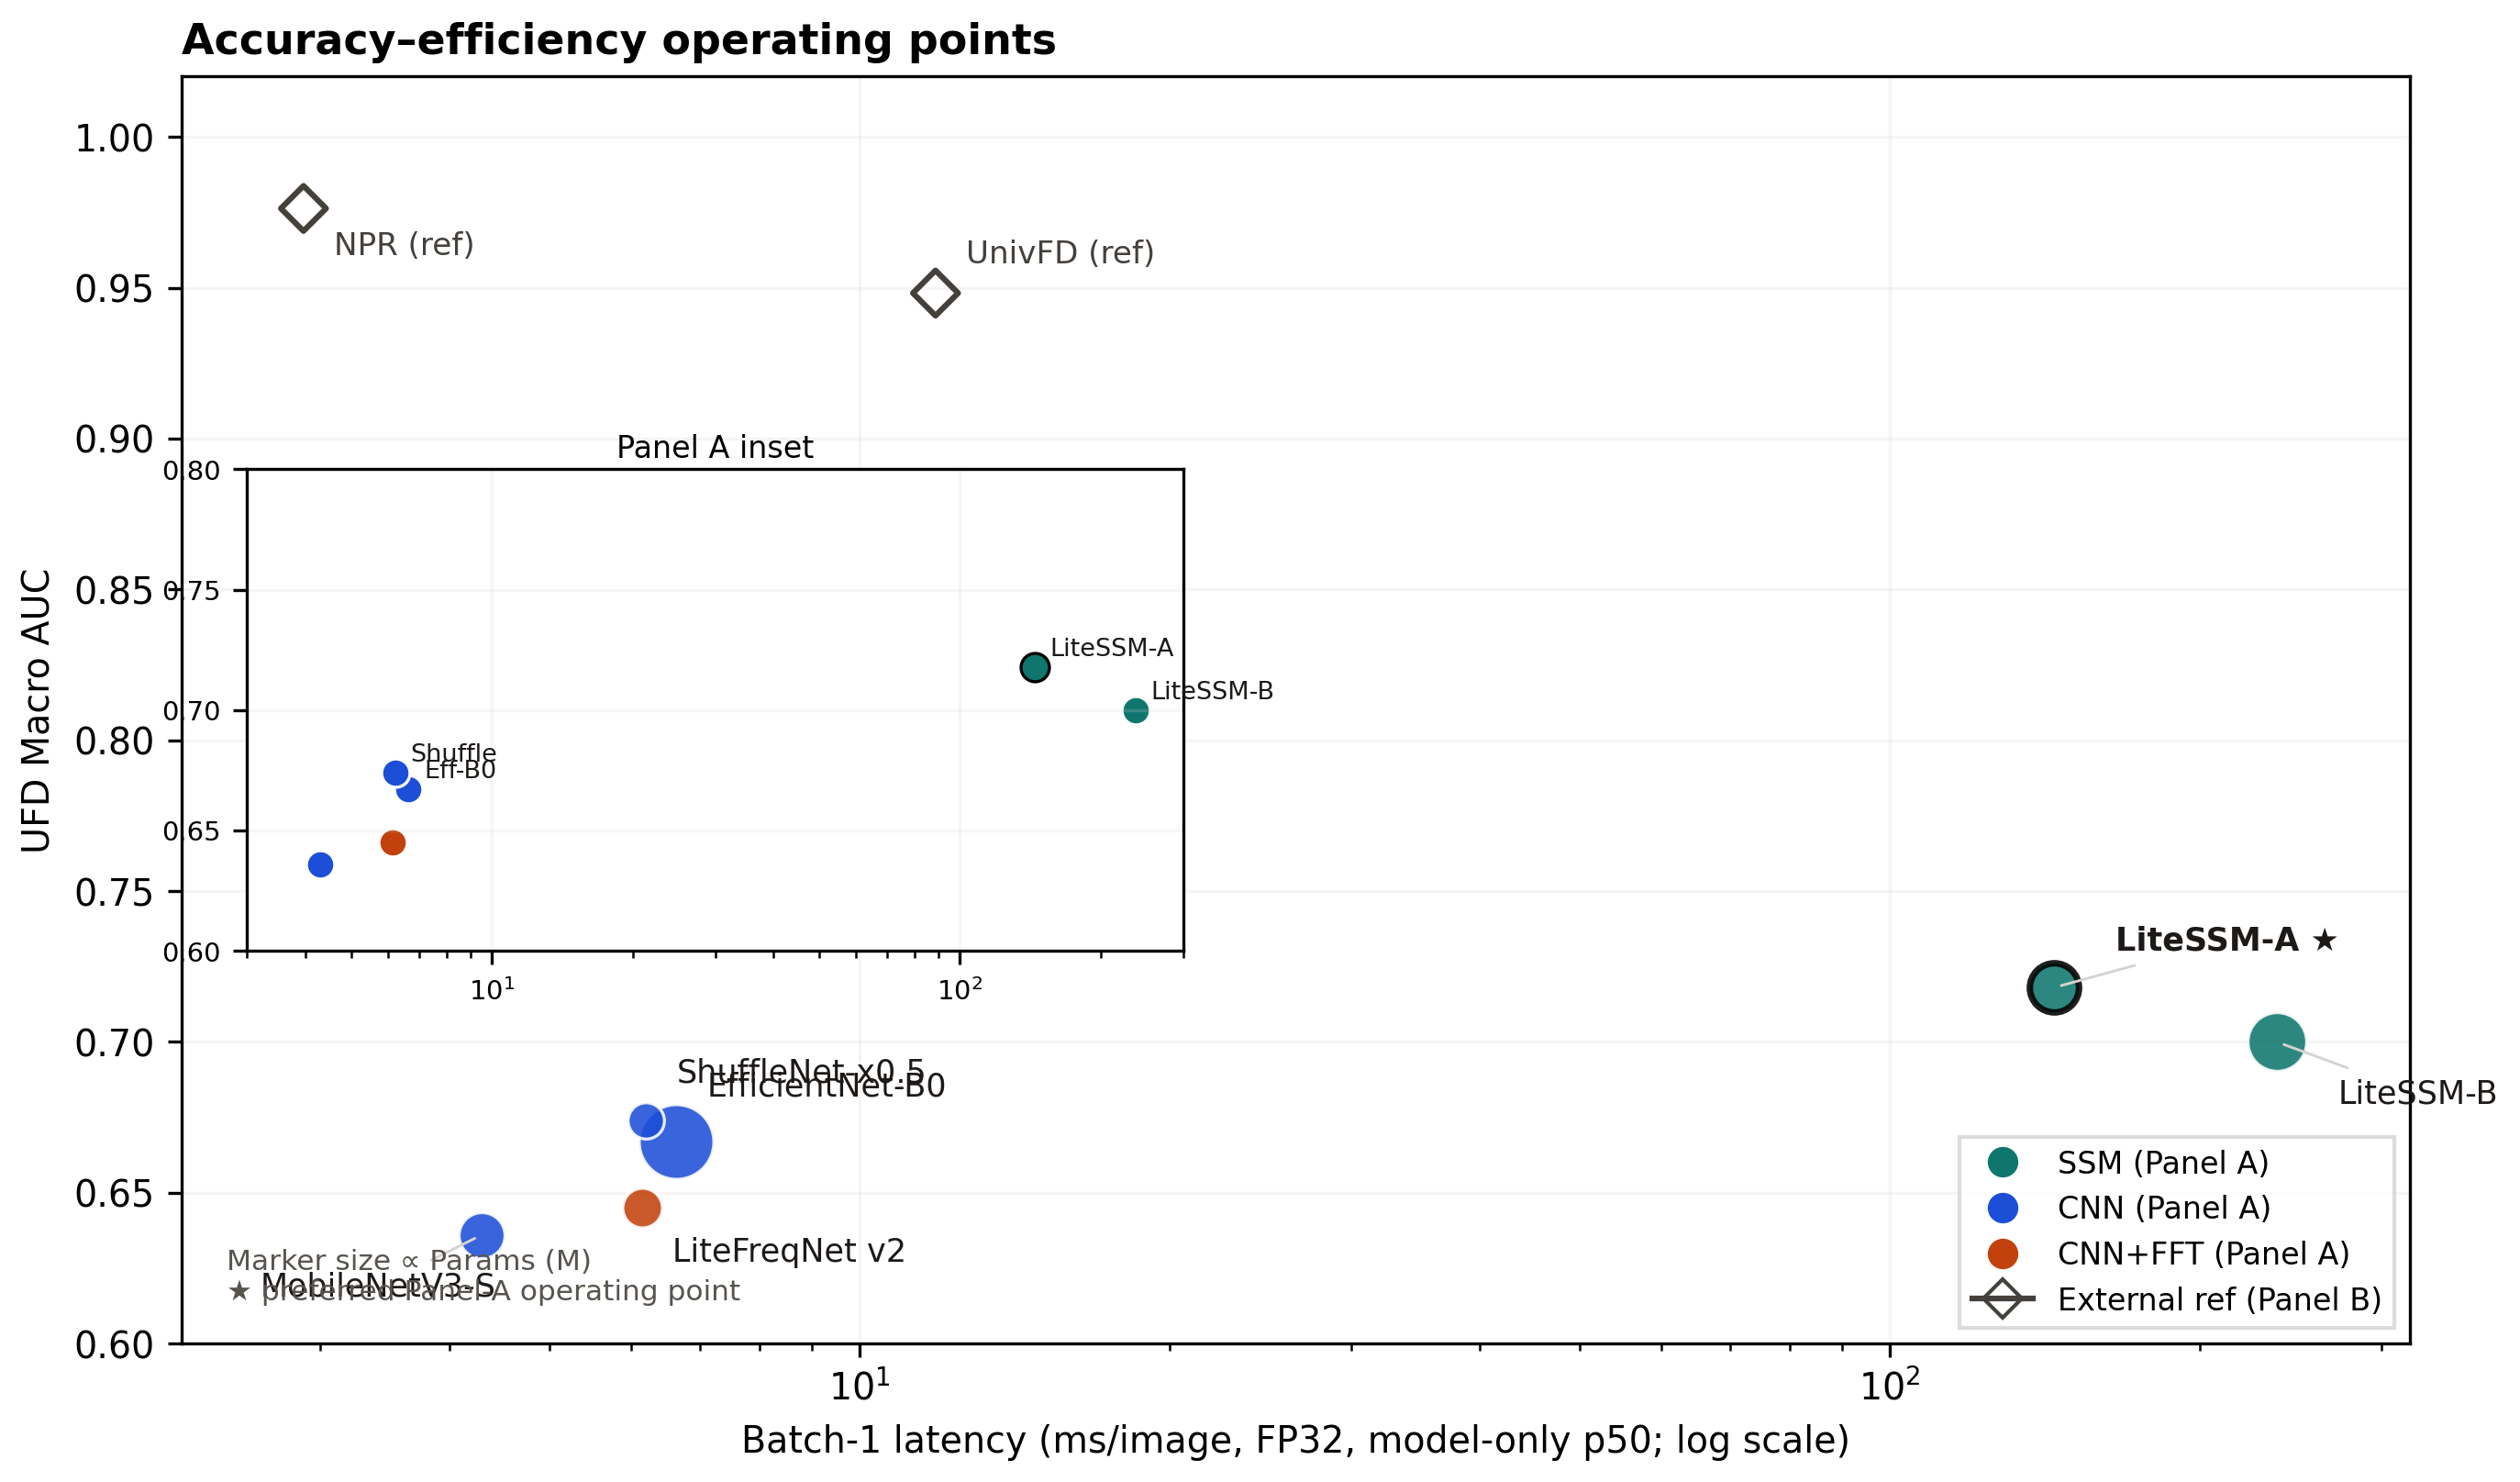
\includegraphics[width=0.92\textwidth]{figures/fig2_pareto_ufd_macro.png}
\caption{Accuracy--efficiency plot using UFD Macro AUC versus batch-1 latency (ms/image, FP32, model-only p50; log $x$-axis).
Filled markers: Panel~A; hollow diamonds: Panel~B references; marker size scales with Params.
The main panel keeps the full $[0.60,1.00]$ Macro range so Panel~B absolute gaps remain visible; the inset magnifies the Panel~A band $[0.60,0.80]$.
LiteSSM-A is marked as the preferred Panel~A operating point (highest Macro, not lowest latency).\label{fig:pareto}}
\end{figure}

\begin{table}[H]
\caption{Operating metrics at a fixed decision threshold.
For Panel~A, the threshold is fitted on the validation set by Youden's $J$ and applied unchanged to ID test and UFD (pooled).
For Panel~B references we report a fixed score threshold of $0.5$ (not recipe-matched Youden).
Bal.\ Acc.\ $=$ $(\mathrm{Sens}+\mathrm{Spec})/2$.\label{tab:operate}}
\scriptsize
\setlength{\tabcolsep}{3.2pt}
\begin{tabularx}{\textwidth}{@{}P{2.15cm}l c *{4}{R}@{}}
\toprule
\textbf{Model} & \textbf{Split} & \textbf{Thr} & \textbf{Bal.} & \textbf{F1} & \textbf{Sens.} & \textbf{Spec.} \\
\midrule
LiteSSM-A & ID & 0.43 & 0.863 & 0.870 & 0.920 & 0.805 \\
LiteSSM-A & UFD pooled & 0.43 & 0.676 & 0.604 & 0.494 & 0.859 \\
EfficientNet-B0 & ID & 0.54 & 0.805 & 0.818 & 0.875 & 0.735 \\
EfficientNet-B0 & UFD pooled & 0.54 & 0.617 & 0.534 & 0.440 & 0.793 \\
LiteFreqNet~v2 & ID & 0.94 & 0.823 & 0.829 & 0.860 & 0.785 \\
LiteFreqNet~v2 & UFD pooled & 0.94 & 0.603 & 0.517 & 0.426 & 0.781 \\
NPR (ref) & ID & 0.50 & 0.867 & 0.862 & 0.830 & 0.905 \\
NPR (ref) & UFD pooled & 0.50 & 0.945 & 0.945 & 0.943 & 0.947 \\
UnivFD (ref) & ID & 0.50 & 0.510 & 0.222 & 0.140 & 0.880 \\
UnivFD (ref) & UFD pooled & 0.50 & 0.818 & 0.781 & 0.650 & 0.986 \\
\bottomrule
\end{tabularx}
\end{table}

\subsection{Within-ID Performance by Content Domain}
\label{sec:domain}

Table~\ref{tab:domain} and Figure~\ref{fig:domain} report domain-wise AUCs on the ID test split.
CelebA-HQ AUCs were near saturation for all models (0.992--0.999).
Bedroom AUCs were substantially lower and separated detectors: SSM models reached $\approx$0.81, EfficientNet-B0 0.777, and remaining compact CNNs 0.677--0.713.
Aggregate ID improvements therefore primarily reflect gains on the harder bedroom domain.

\begin{figure}[H]
\centering
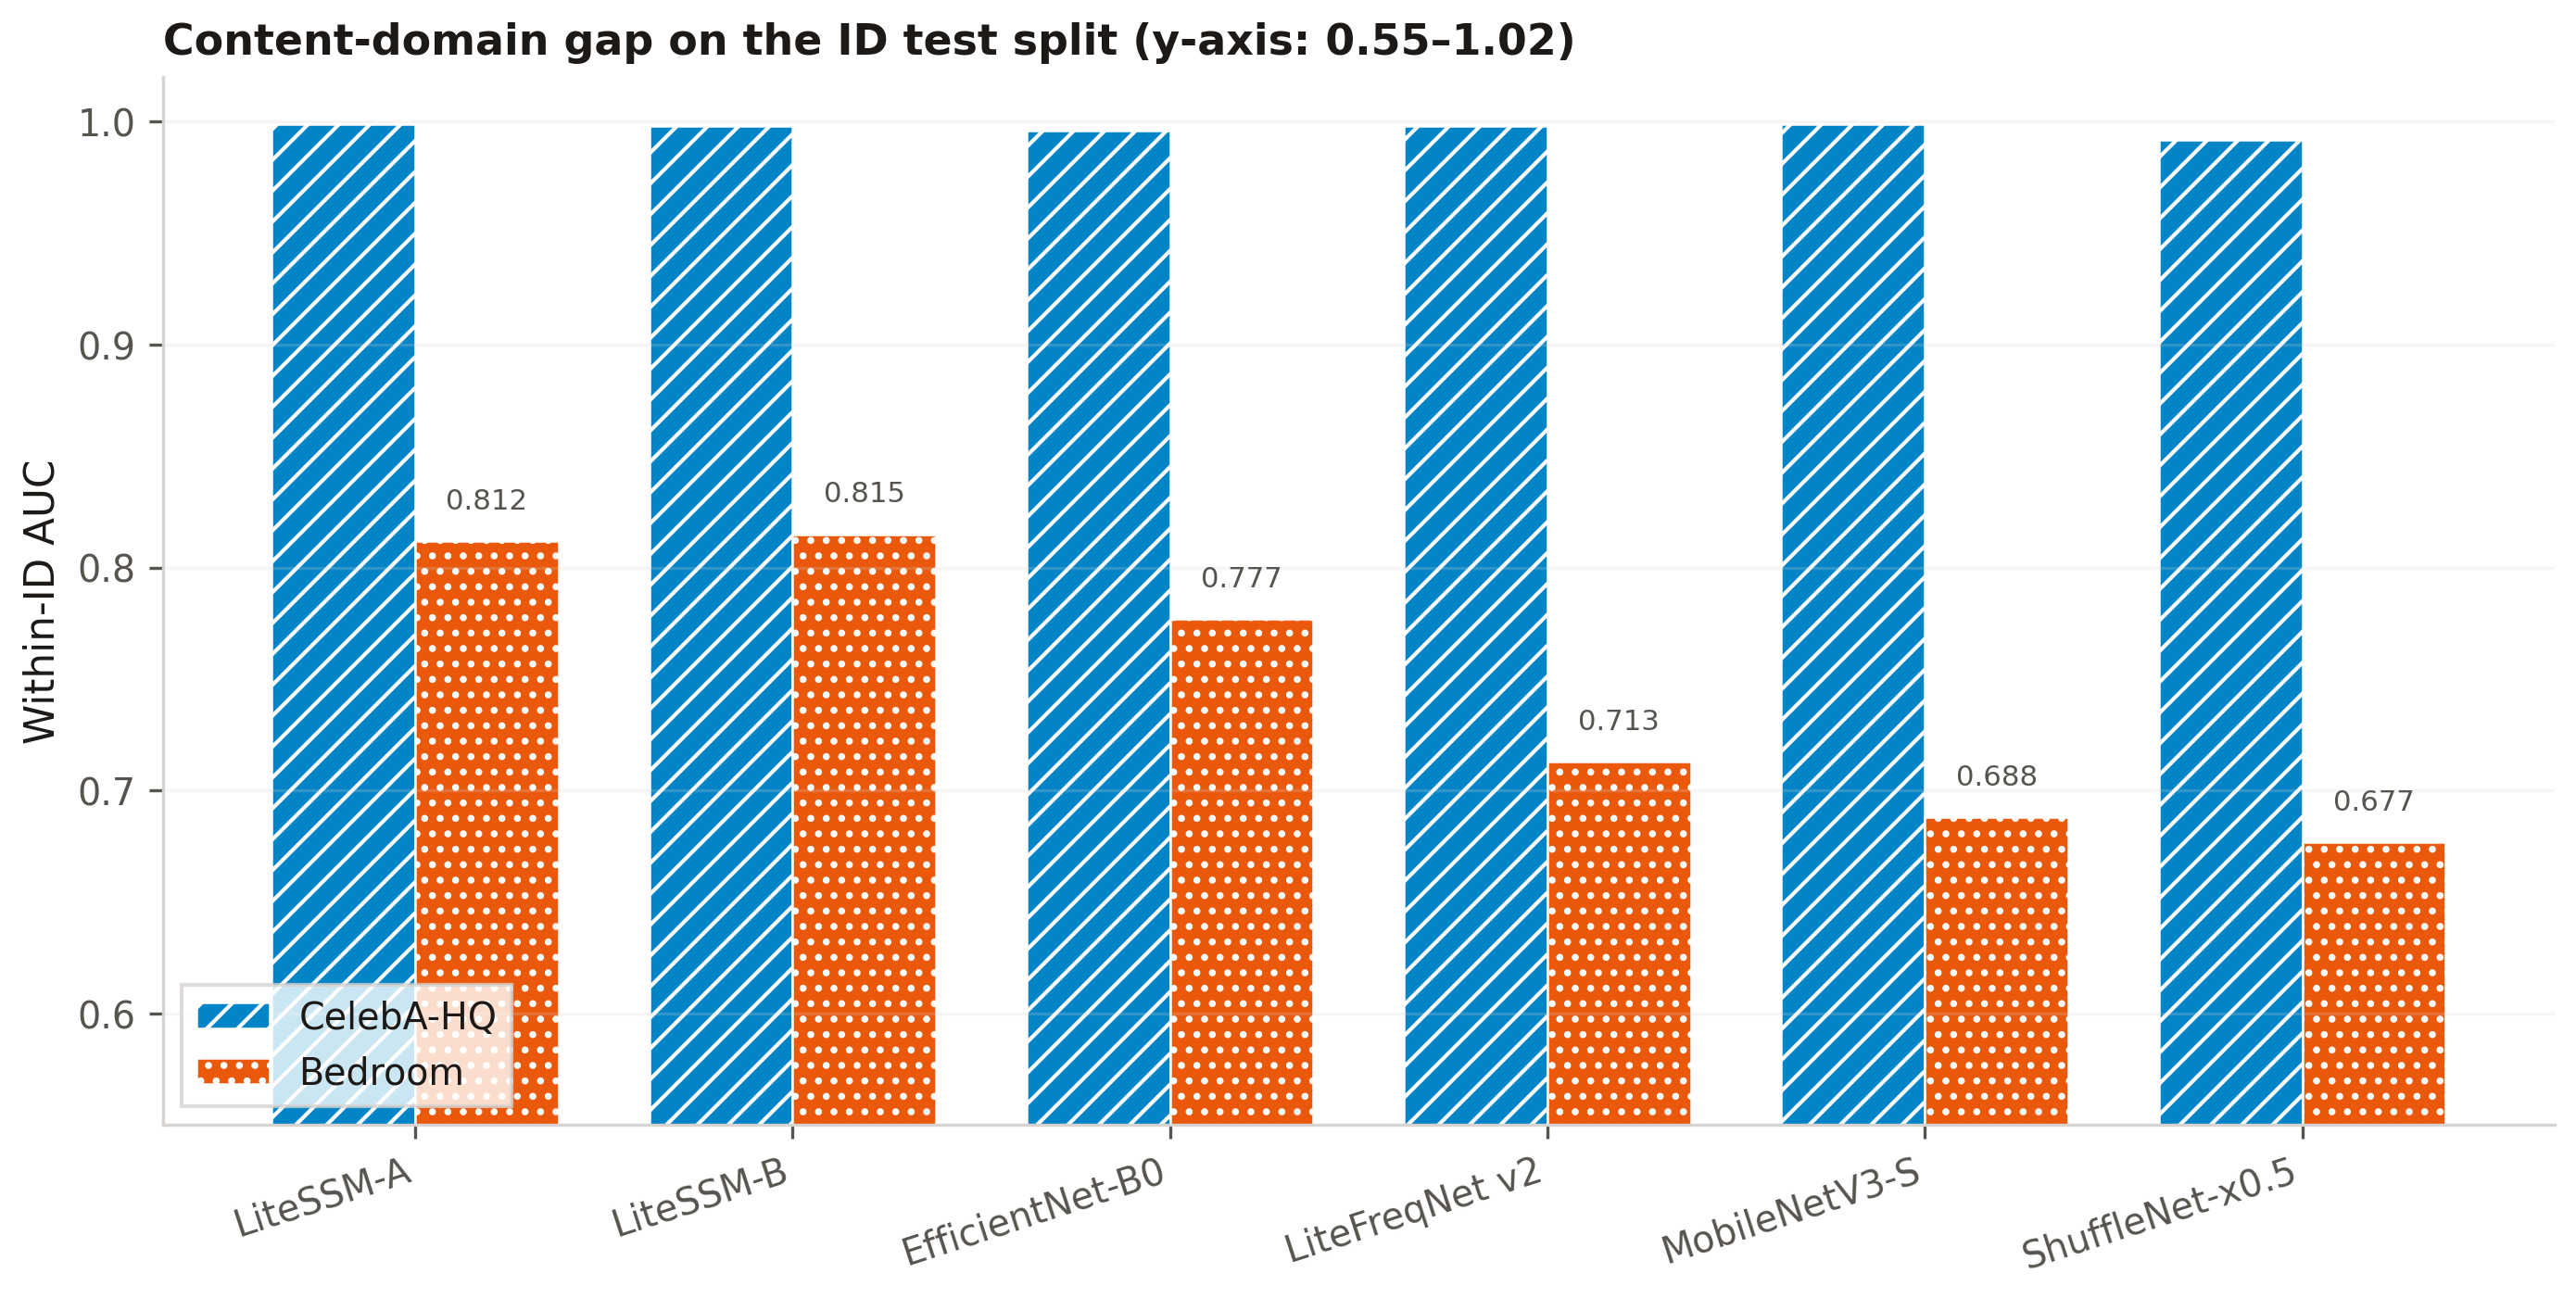
\includegraphics[width=0.95\textwidth]{figures/fig_domain_gap.png}
\caption{Within-ID AUCs by content domain.
CelebA-HQ is near saturation for all Panel~A models; bedroom AUC is the discriminative axis.\label{fig:domain}}
\end{figure}

\begin{table}[H]
\caption{Within-ID AUCs by content domain.\label{tab:domain}}
\scriptsize
\setlength{\tabcolsep}{4pt}
\begin{tabularx}{\textwidth}{@{}P{2.4cm}*{4}{R}@{}}
\toprule
\textbf{Model} & \textbf{ID} & \textbf{CelebA-HQ} & \textbf{Bedroom} & \textbf{Gap} \\
\midrule
LiteSSM-A & 0.946 & 0.999 & 0.812 & 0.187 \\
LiteSSM-B & 0.945 & 0.998 & 0.815 & 0.183 \\
EfficientNet-B0 & 0.929 & 0.996 & 0.777 & 0.219 \\
LiteFreqNet~v2 & 0.906 & 0.998 & 0.713 & 0.285 \\
MobileNetV3-Small & 0.890 & 0.999 & 0.688 & 0.311 \\
ShuffleNetV2-x0.5 & 0.880 & 0.992 & 0.677 & 0.315 \\
\bottomrule
\end{tabularx}
\end{table}

\subsection{Per-Generator Evaluation on UniversalFakeDetect}
\label{sec:ufd}

Table~\ref{tab:ufd} reports per-subset AUCs on UFD~\cite{ojha2023ufd}.
SSM detectors obtain higher Macro averages than the CNN/frequency suite.
Generator identity dominates architecture: Glide subsets are comparatively easy, LDM subsets are weaker, and rankings change across columns.
\textbf{DALL·E remained close to chance for every Panel~A detector (0.451--0.519)}, including both SSMs; the failure is not specific to LiteFreqNet.
Table~\ref{tab:ufd-ext} places the same frozen UFD subsets next to Panel~B pretrained references: UnivFD and NPR remain strong on DALL·E (0.969 / 0.990) and reach substantially higher Macro AUCs.
This contrast indicates a \emph{protocol/panel gap} rather than absolute undetectability of DALL·E under every training paradigm; Panel~B scores are contextual and are \emph{not} ranked against Panel~A under a shared recipe.
Figure~\ref{fig:heatmap} visualizes the Panel~A UFD generator--model matrix.

\begin{table}[H]
\caption{Per-generator AUCs on UFD (400 real + 400 fake per subset).
Macro $=$ equal-weight mean; Min $=$ worst-subset AUC.
Abbreviations: G10/G27/G50 $=$ Glide$_{100,10}$ / Glide$_{100,27}$ / Glide$_{50,27}$; L100/L200/Lcfg $=$ LDM$_{100}$ / LDM$_{200}$ / LDM$_{200,\mathrm{cfg}}$.\label{tab:ufd}}
\scriptsize
\setlength{\tabcolsep}{2.6pt}
\begin{tabularx}{\textwidth}{@{}P{2.05cm}*{10}{R}@{}}
\toprule
\textbf{Model} & \textbf{DALL·E} & \textbf{G10} & \textbf{G27} & \textbf{G50} & \textbf{Guid.} & \textbf{L100} & \textbf{L200} & \textbf{Lcfg} & \textbf{Macro} & \textbf{Min} \\
\midrule
LiteSSM-A & 0.504 & 0.878 & 0.855 & 0.889 & 0.766 & 0.656 & 0.634 & 0.565 & 0.718 & 0.504 \\
LiteSSM-B & 0.483 & 0.859 & 0.831 & 0.868 & 0.788 & 0.622 & 0.611 & 0.535 & 0.700 & 0.483 \\
EfficientNet-B0 & 0.519 & 0.773 & 0.782 & 0.795 & 0.720 & 0.613 & 0.577 & 0.557 & 0.667 & 0.519 \\
LiteFreqNet~v2 & 0.451 & 0.786 & 0.763 & 0.808 & 0.678 & 0.594 & 0.551 & 0.531 & 0.645 & 0.451 \\
MobileNetV3-S & 0.455 & 0.746 & 0.739 & 0.770 & 0.656 & 0.621 & 0.580 & 0.518 & 0.636 & 0.455 \\
ShuffleNet-x0.5 & 0.467 & 0.805 & 0.802 & 0.835 & 0.755 & 0.617 & 0.570 & 0.537 & 0.674 & 0.467 \\
\bottomrule
\end{tabularx}
\end{table}

\begin{table}[H]
\caption{External reference (Panel~B) per-generator AUCs on the same frozen UFD subsets.
Scores are inference-only with public checkpoints and native preprocessing; they contextualize the remaining gap to large-scale pretrained detectors and are not protocol-matched competitors.
Abbreviations follow Table~\ref{tab:ufd}.\label{tab:ufd-ext}}
\scriptsize
\setlength{\tabcolsep}{2.8pt}
\begin{tabularx}{\textwidth}{@{}P{1.7cm}*{9}{R}@{}}
\toprule
\textbf{Detector} & \textbf{DALL·E} & \textbf{G10} & \textbf{G27} & \textbf{G50} & \textbf{Guid.} & \textbf{L100} & \textbf{L200} & \textbf{Lcfg} & \textbf{Macro} \\
\midrule
UnivFD~\cite{ojha2023ufd} & 0.969 & 0.942 & 0.956 & 0.962 & 0.861 & 0.989 & 0.992 & 0.916 & 0.948 \\
NPR~\cite{tan2024npr} & 0.990 & 0.995 & 0.995 & 0.996 & 0.837 & 0.999 & 0.998 & 0.999 & 0.976 \\
\bottomrule
\end{tabularx}
\end{table}

\begin{figure}[H]
\centering
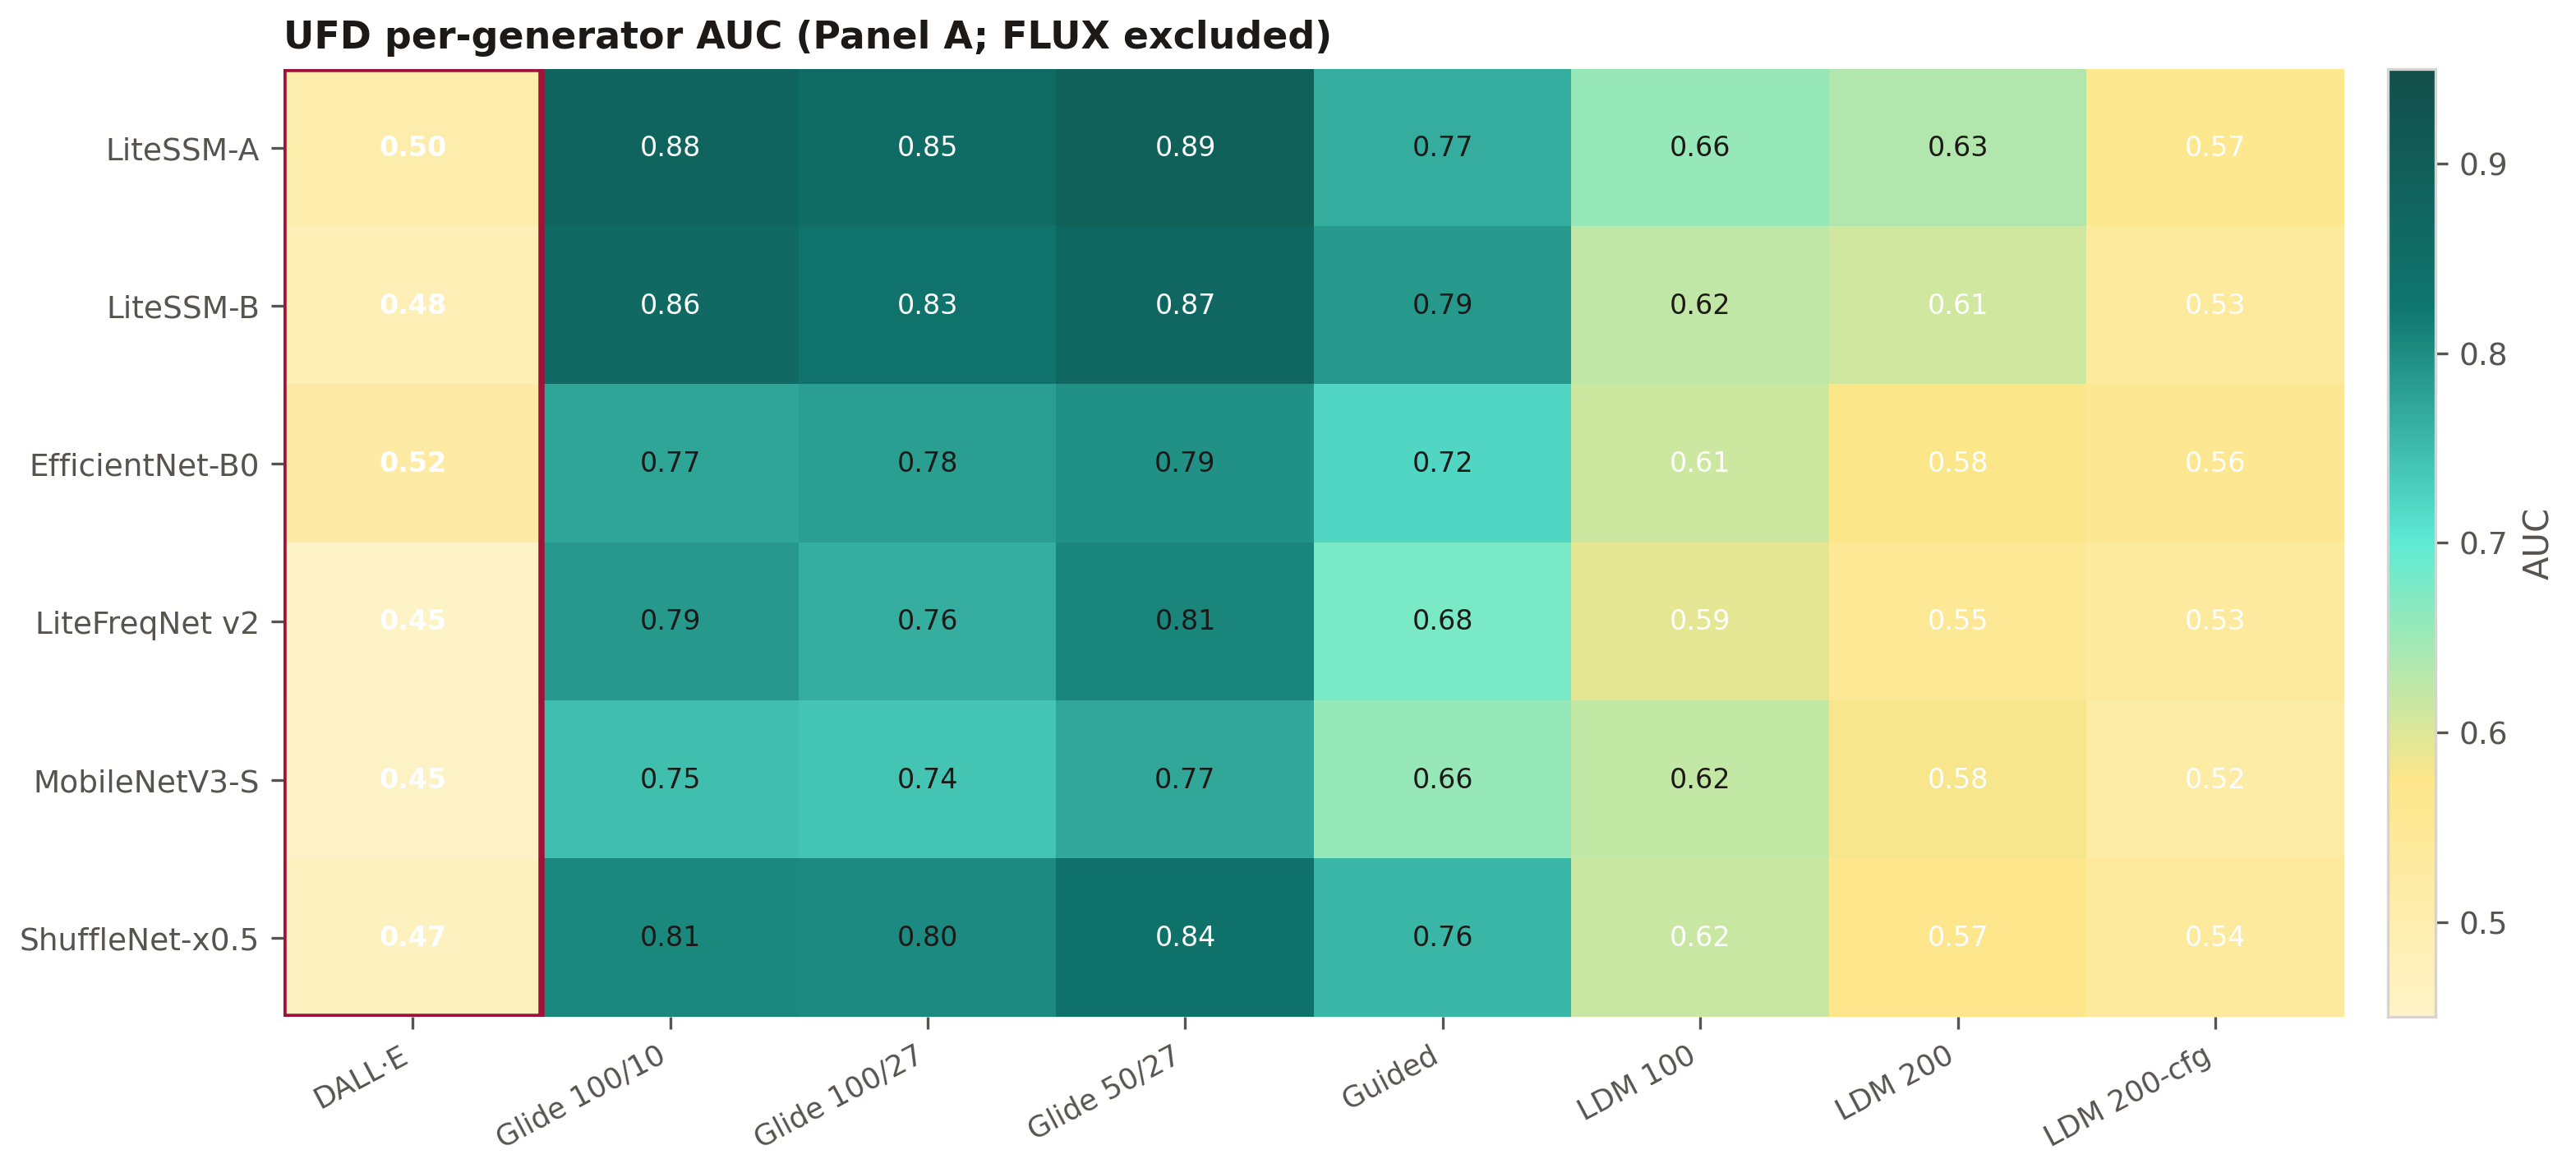
\includegraphics[width=0.98\textwidth]{figures/fig3_generator_heatmap.png}
\caption{Generator--model AUC heatmap for UFD subsets (Panel~A).
The outlined DALL·E column remains near chance for every training-matched compact model.\label{fig:heatmap}}
\end{figure}

Figure~\ref{fig:dalle-diag} diagnoses the DALL·E failure at the score level.
On Glide$_{100,10}$, Panel~A fake/real score mass separates; on DALL·E the two classes largely overlap for LiteSSM-A and EfficientNet-B0, whereas NPR retains clear separation.
A full causal diagnosis would require matched acquisition metadata and spectral decomposition; the present evidence establishes a protocol-level boundary rather than a mechanistic explanation.

\begin{figure}[H]
\centering
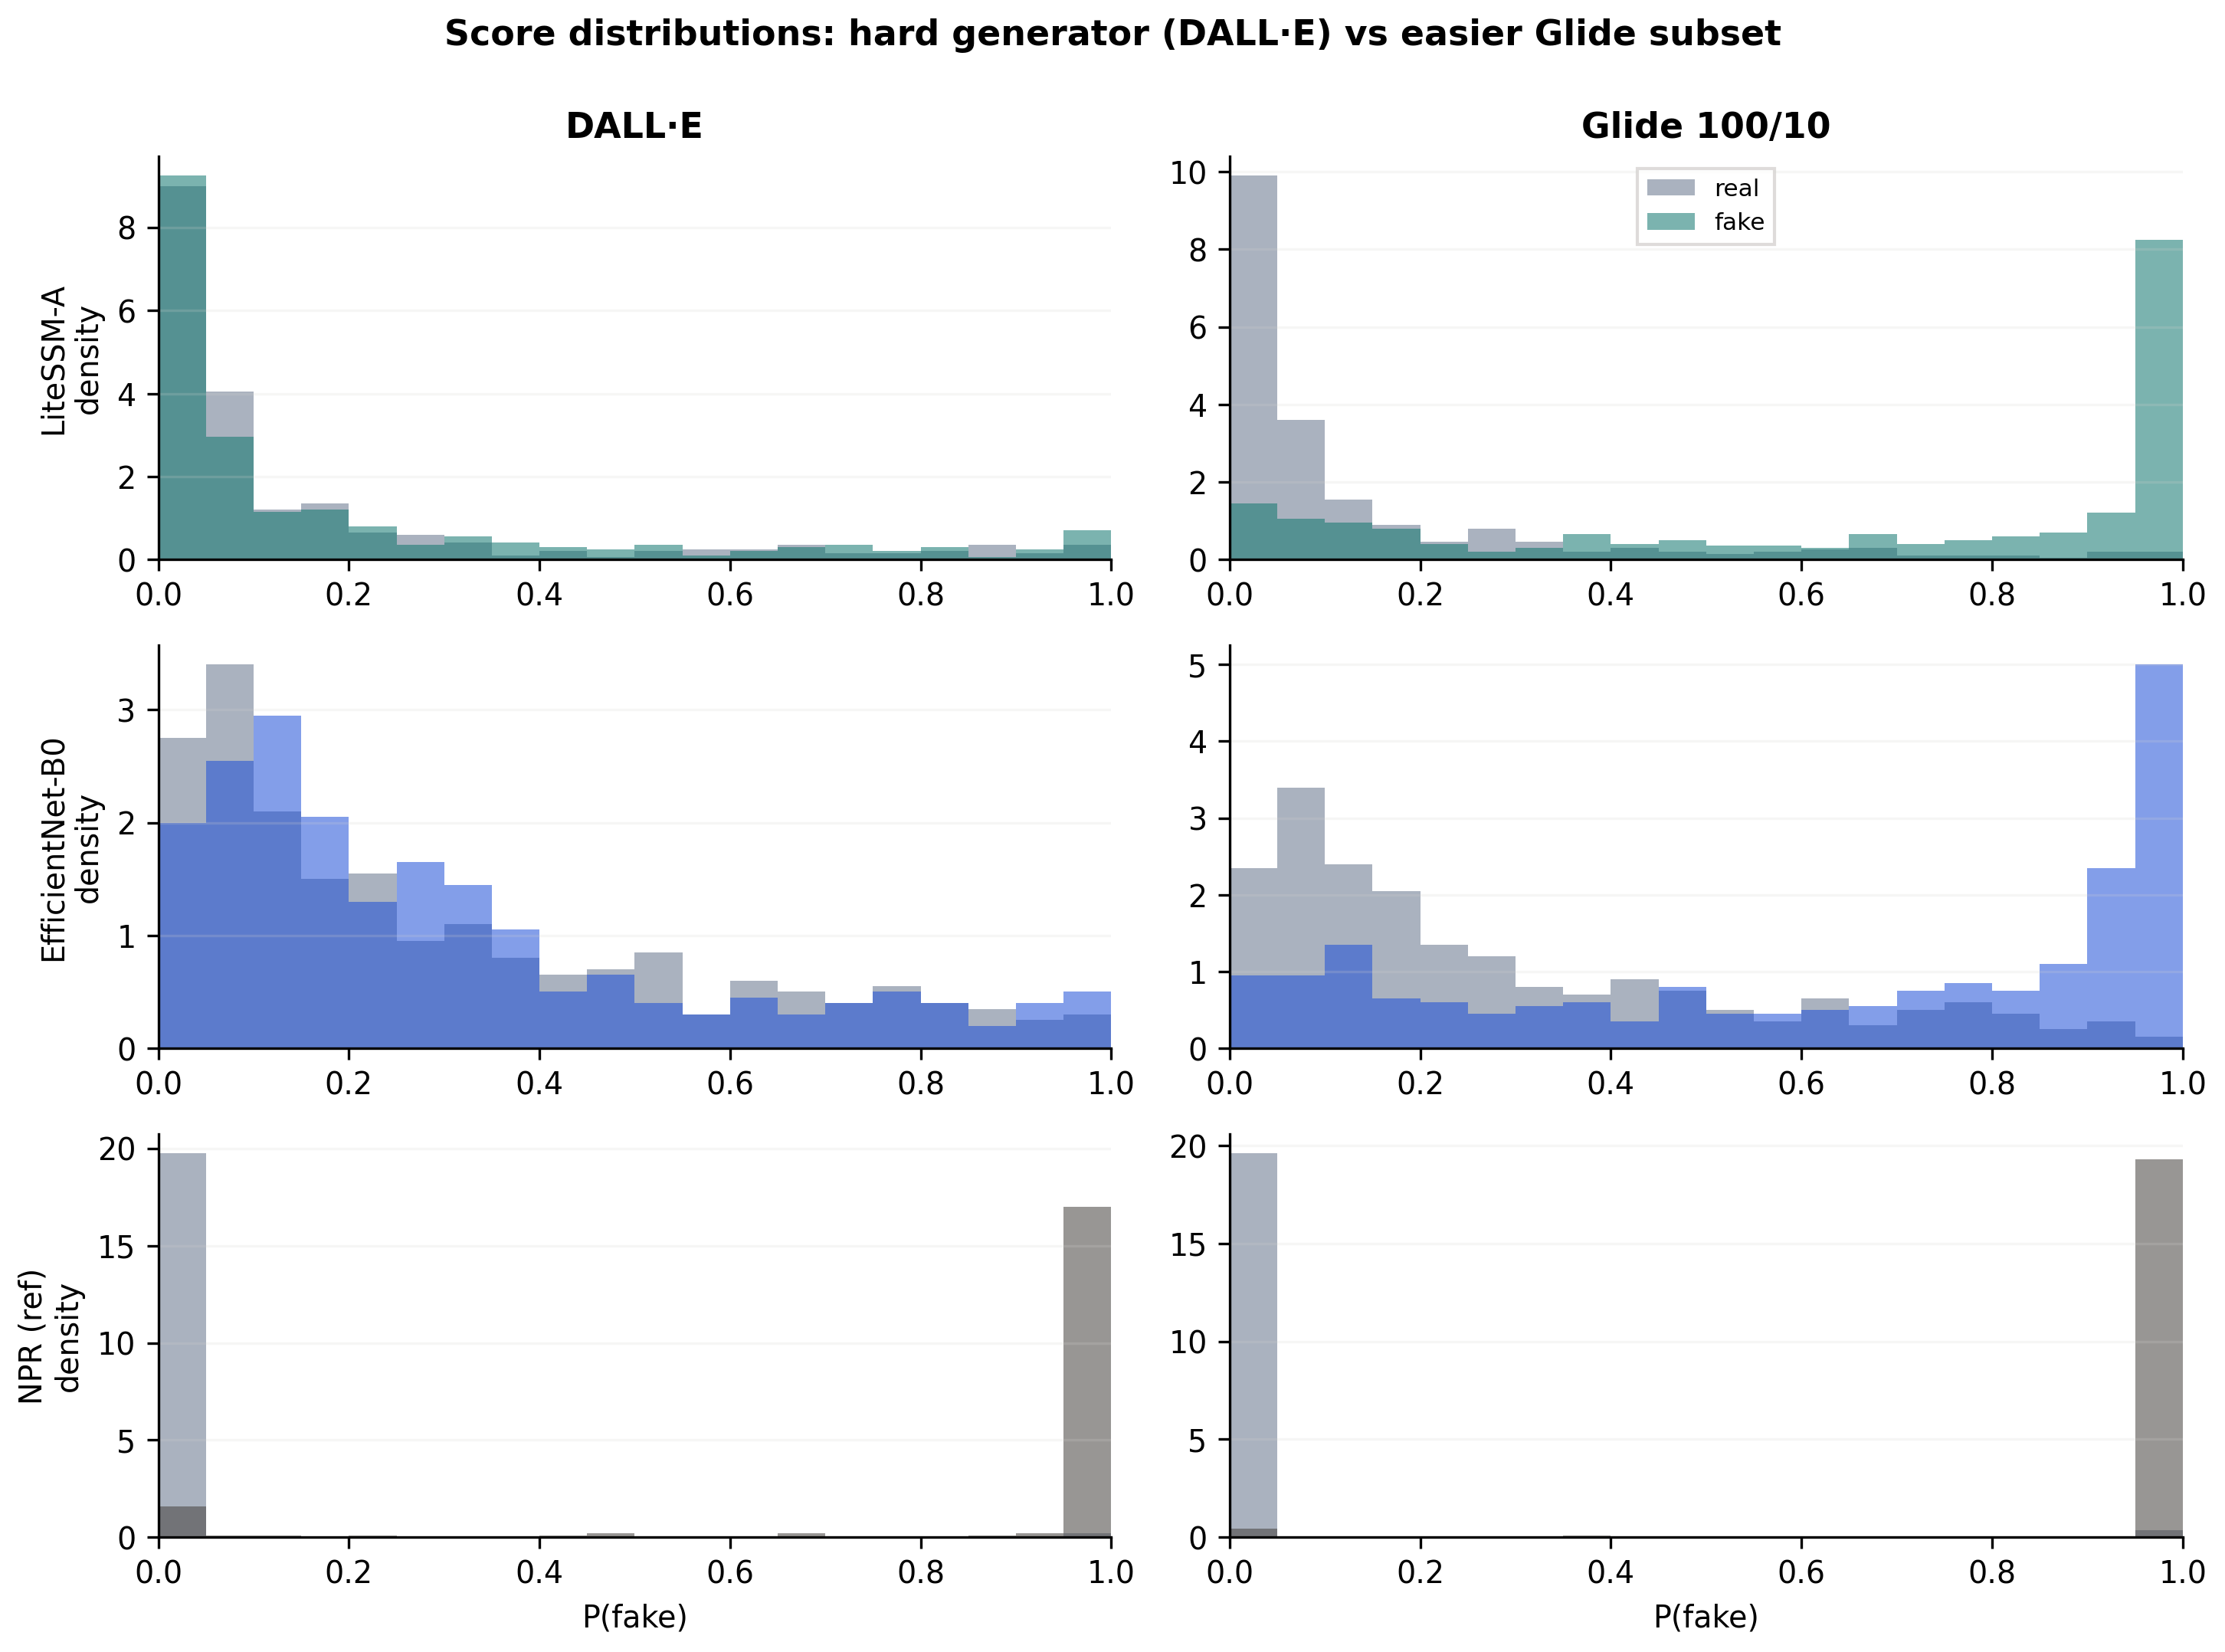
\includegraphics[width=0.98\textwidth]{figures/fig_dalle_score_diag.png}
\caption{Score distributions on UFD DALL·E versus Glide$_{100,10}$ for LiteSSM-A, EfficientNet-B0, and NPR (ref).
Panel~A overlap on DALL·E explains near-chance AUCs; NPR remains separated under a different training paradigm.\label{fig:dalle-diag}}
\end{figure}

\subsection{Robustness under JPEG Q70 Recompression}
\label{sec:jpeg}

Table~\ref{tab:jpeg} compares clean ID AUC with JPEG $Q=70$.
Absolute AUC changes were at most \textbf{0.003} for all models.
Figure~\ref{fig:jpeg-forest} plots paired-bootstrap $\Delta$AUC with 95\% CIs; all intervals include or hug zero, and LiteFreqNet~v2 shows no unique robustness advantage.
The shared observation is stability under the evaluated JPEG Q70 setting, not frequency-module superiority.
A multi-quality absolute-AUC sweep ($Q\in\{95,85,70\}$) remains in Appendix~\ref{app:jpeg}.

\begin{figure}[H]
\centering
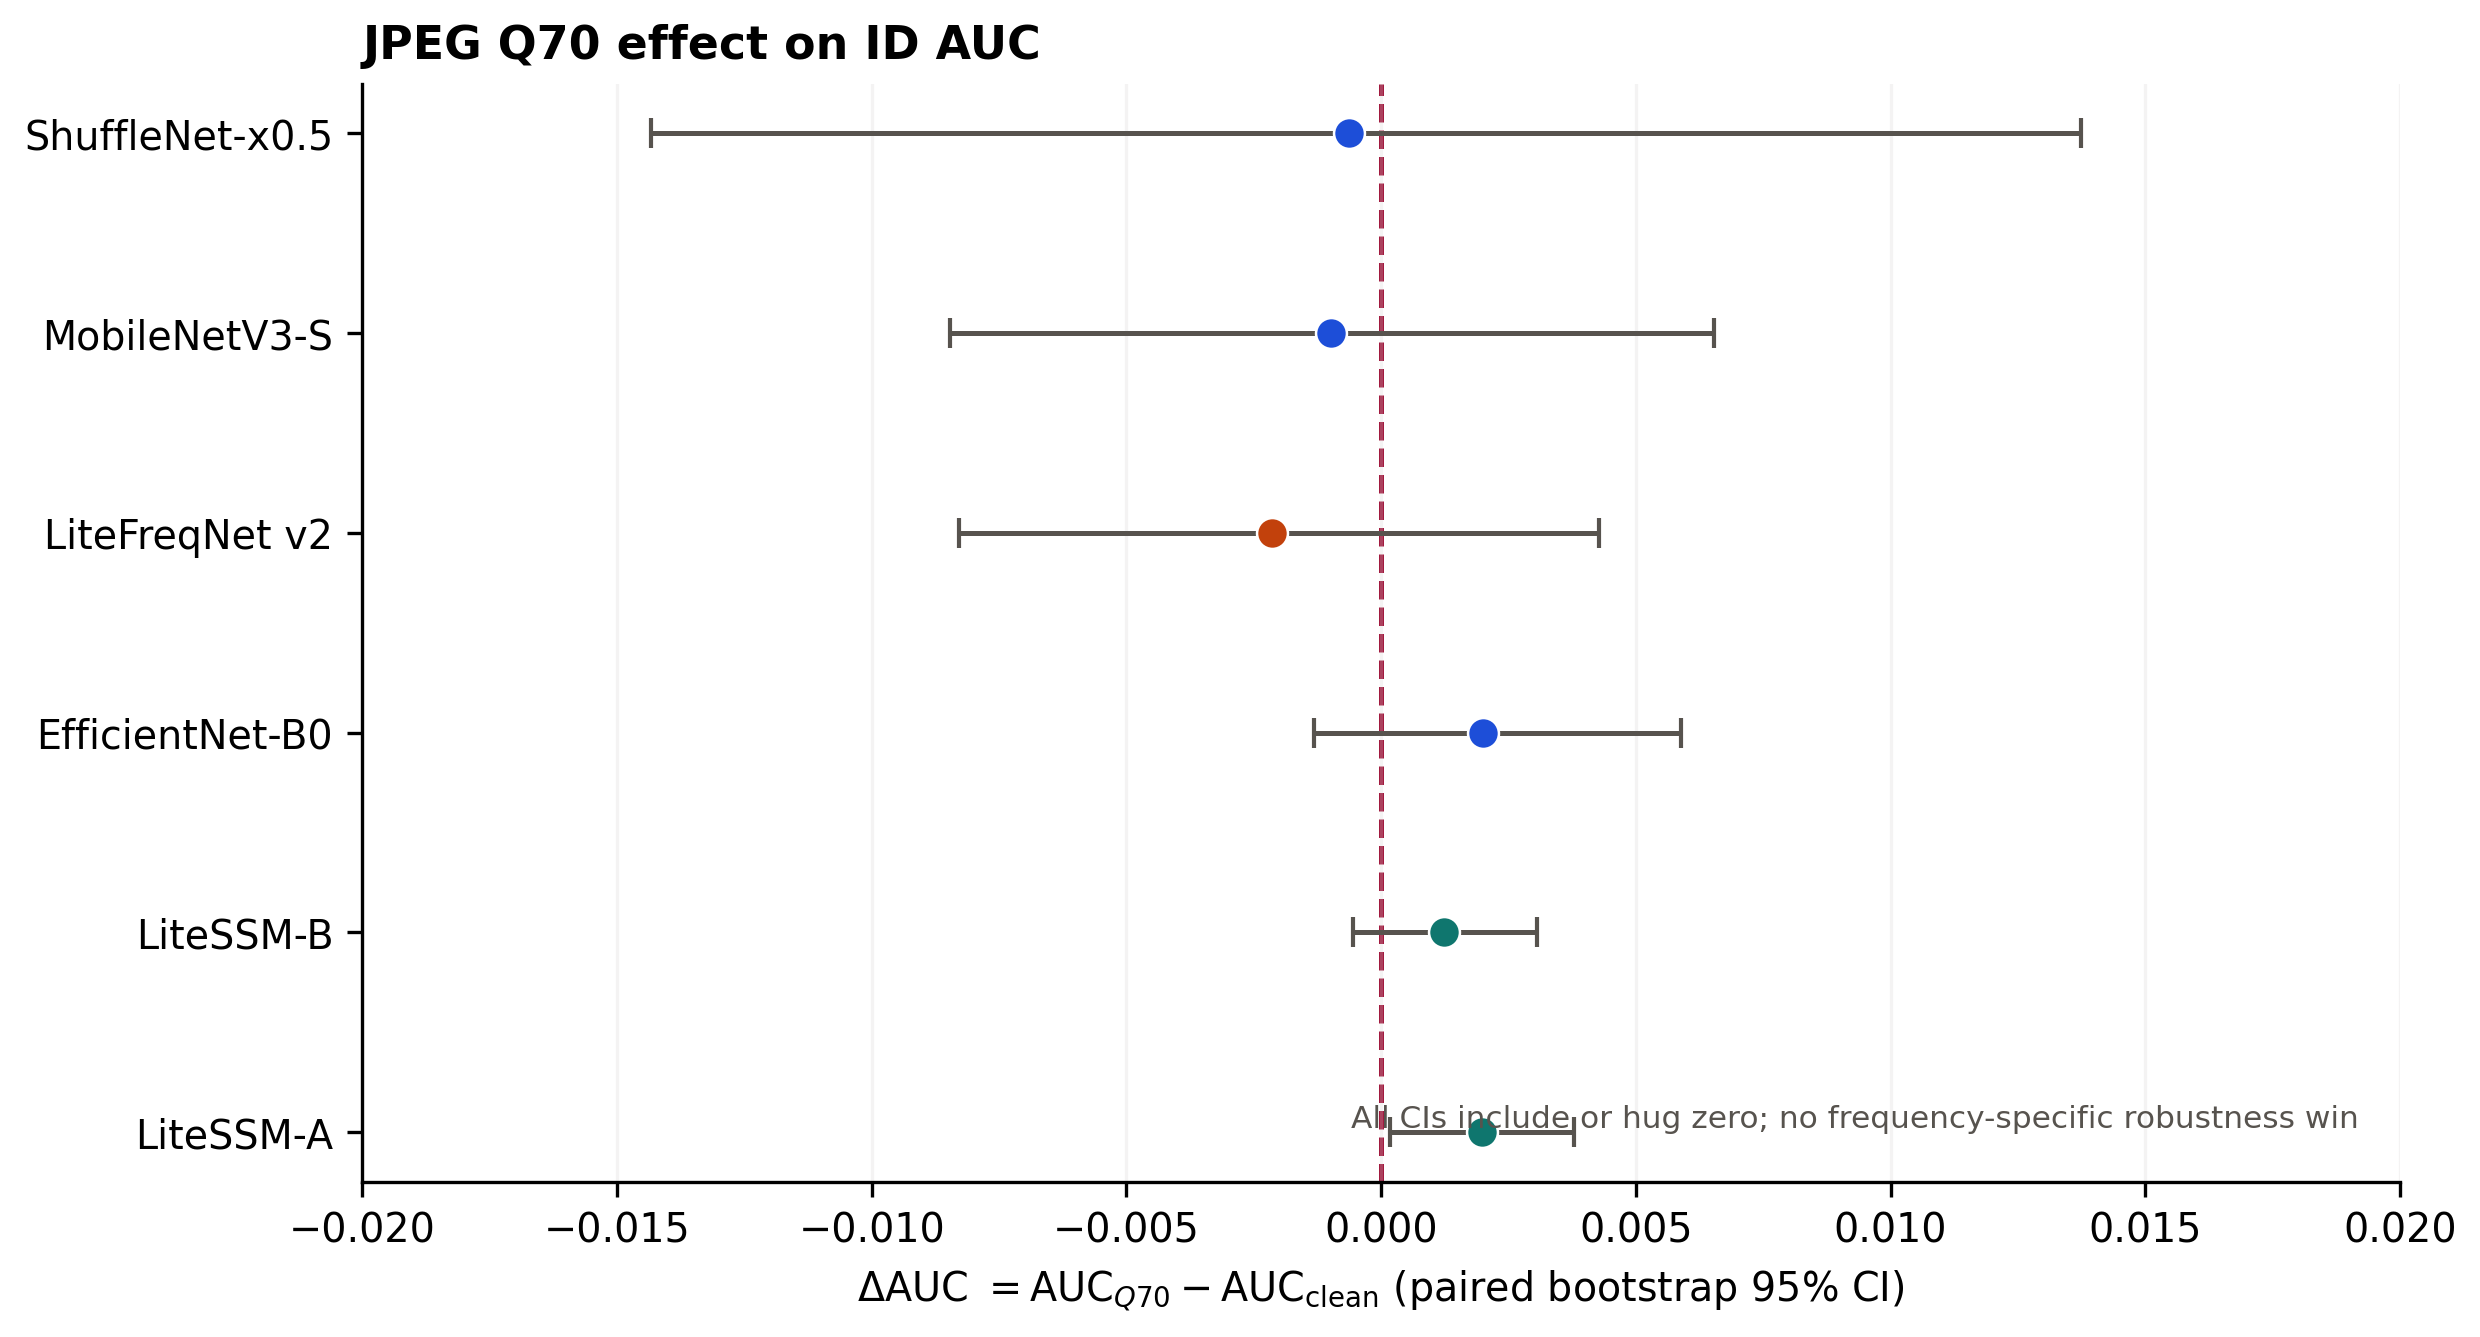
\includegraphics[width=0.92\textwidth]{figures/fig_jpeg_delta_forest.png}
\caption{Forest plot of ID $\Delta$AUC $=\mathrm{AUC}_{Q70}-\mathrm{AUC}_{\mathrm{clean}}$ with paired bootstrap 95\% CIs ($B=1000$, seed~42).
The dashed line marks zero effect.\label{fig:jpeg-forest}}
\end{figure}

\begin{table}[H]
\caption{ID AUC under JPEG Q70 recompression.\label{tab:jpeg}}
\scriptsize
\setlength{\tabcolsep}{4pt}
\begin{tabularx}{\textwidth}{@{}P{2.4cm}*{4}{R}@{}}
\toprule
\textbf{Model} & \textbf{Clean} & \textbf{Q70} & \textbf{$\Delta$AUC} & \textbf{$\Delta$CI95} \\
\midrule
LiteSSM-A & 0.946 & 0.948 & $+0.002$ & $[+0.000,\ +0.004]$ \\
LiteSSM-B & 0.945 & 0.946 & $+0.001$ & $[-0.001,\ +0.003]$ \\
EfficientNet-B0 & 0.929 & 0.931 & $+0.002$ & $[-0.001,\ +0.006]$ \\
LiteFreqNet~v2 & 0.906 & 0.904 & $-0.002$ & $[-0.008,\ +0.004]$ \\
MobileNetV3-Small & 0.890 & 0.889 & $-0.001$ & $[-0.009,\ +0.007]$ \\
ShuffleNetV2-x0.5 & 0.880 & 0.879 & $-0.001$ & $[-0.014,\ +0.014]$ \\
\bottomrule
\end{tabularx}
\end{table}

\subsection{Ablation and Frequency-Module Transferability}

Replacing early concatenation with gated residual fusion recovered usable thresholds after a probability-collapse failure in the initial LiteFreq design; LiteFreqNet~v2 is retained in the main tables.
Table~\ref{tab:freq-abl} summarizes frequency-branch ablations under the bake-off protocol.
Attaching the frequency branch to SSM backbones slightly reduced ID and OOD Pooled AUC; removing the frequency branch from LiteFreqNet likewise hurts ID/OOD Pooled.
Frequency-branch variants for SSM backbones (and the LiteFreq no-frequency control) were evaluated with OOD Pooled AUC; \textbf{UFD Macro was not recomputed for these ablations}.
Frequency injection was therefore not a transferable free upgrade across architectures in this protocol.

\begin{table}[H]
\caption{Frequency-module ablation under the locked bake-off protocol.
UFD Macro is reported only for primary main-table checkpoints; ablation rows use ID and OOD Pooled only.\label{tab:freq-abl}}
\scriptsize
\setlength{\tabcolsep}{4pt}
\begin{tabularx}{\textwidth}{@{}P{3.2cm}*{3}{R}@{}}
\toprule
\textbf{Model} & \textbf{ID} & \textbf{OOD Pooled} & \textbf{UFD Macro} \\
\midrule
LiteSSM-A & 0.946 & 0.712 & 0.718 \\
LiteSSM-A + freq & 0.937 & 0.696 & -- \\
LiteSSM-B & 0.945 & 0.722 & 0.700 \\
LiteSSM-B + freq & 0.938 & 0.695 & -- \\
LiteFreqNet~v2 & 0.906 & 0.698 & 0.645 \\
LiteFreqNet (no-freq) & 0.857 & 0.648 & -- \\
\bottomrule
\end{tabularx}
\end{table}

An exploratory FLUX evaluation was additionally conducted; however, because the real and synthetic subsets were not content- and acquisition-matched, the results are reported only as supplementary evidence in Appendix~\ref{app:flux} and are \emph{not} used to support architecture-level conclusions.
